\documentclass[11pt,letterpaper]{article}
\usepackage[T1]{fontenc}
\usepackage[utf8]{inputenc}
\usepackage{lmodern}
\usepackage[spanish,es-tabla]{babel}
\decimalpoint
\usepackage[margin=2.3cm]{geometry}
\usepackage{amsmath,amssymb}
\usepackage{booktabs,array}
\usepackage{graphicx}
\usepackage{enumitem}
\usepackage[colorlinks=true,linkcolor=blue!50!black]{hyperref}
\setlist{itemsep=2pt,topsep=3pt}
\setlength{\parindent}{0pt}
\setlength{\parskip}{5pt}
\newcommand{\tht}{\boldsymbol{\theta}}
\newcommand{\norm}[1]{\left\lVert #1\right\rVert}

\title{\vspace{-1.2cm}\textbf{Solucionario del miniproyecto}\\[2pt]
\large Ajuste no lineal: Dogleg, Levenberg--Marquardt y gradiente estoc\'astico\\
\normalsize (documento para el profesor --- no distribuir)}
\date{}
\author{}

\begin{document}
\maketitle
\vspace{-2cm}

\section{Corrida de referencia}
Datos generados con la semilla 2026 (\texttt{generar(2026)}, $n=150$, $\sigma=0.05$).
Los par\'ametros verdaderos son $\tht_{\rm real}=(1.8716,\,1.5420,\,2.9804,\,0.14612)$. El m\'inimo de m\'inimos
cuadrados (referencia de \texttt{least\_squares}, \texttt{lm}, tolerancias $10^{-15}$) es
\[
\tht^\ast=(1.8701,\;1.6937,\;3.0204,\;0.14709),\qquad f^\ast=0.19913,\qquad \hat\sigma=0.0522 .
\]
La suma de cuadrados esperada para ruido puro es $\tfrac12 n\sigma^2=0.1875$, as\'i que $f^\ast$ es coherente con
un buen ajuste. Todo se reproduce con \texttt{python solucion\_referencia.py 2026} (genera las figuras y las
tablas de este documento).

\begin{figure}[h]
\centering
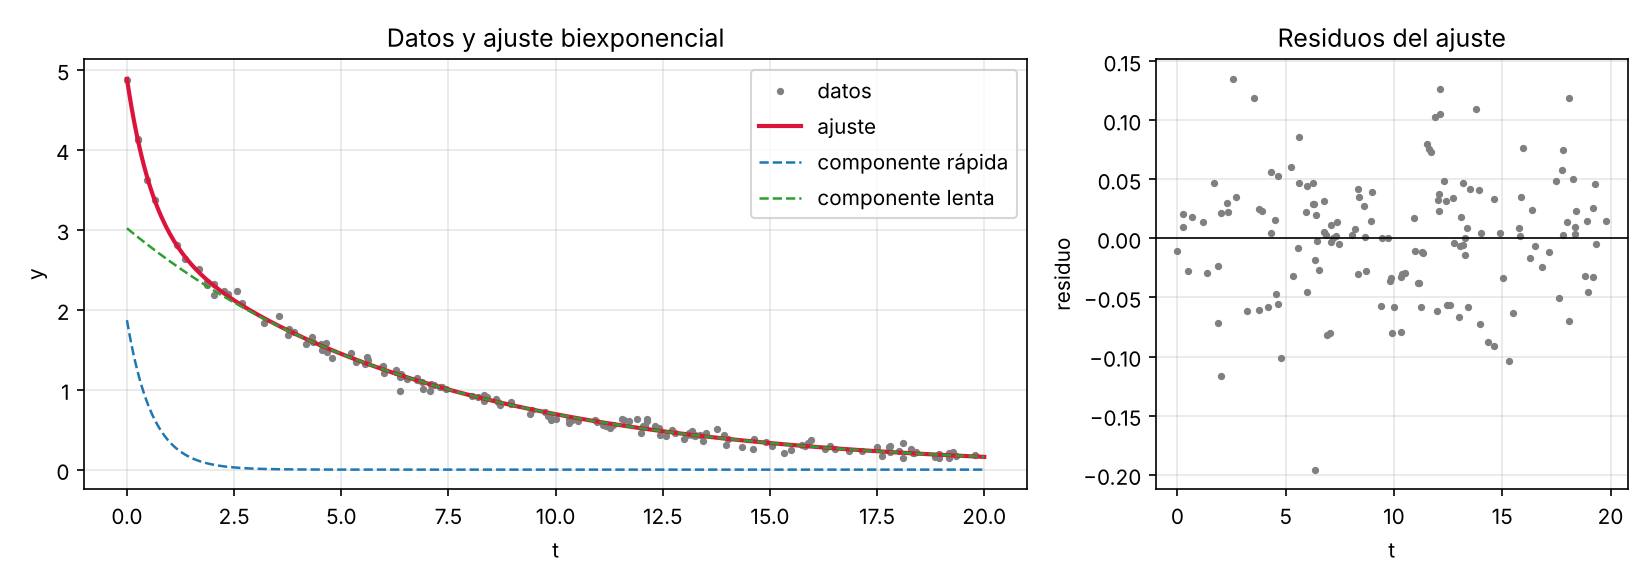
\includegraphics[width=\textwidth]{figs/fig_ajuste.png}
\caption{Datos, ajuste y componentes (izquierda); residuos sin estructura (derecha).}
\end{figure}

\section{Resultados esperados}

\subsection*{Parte A}
Con $e_1=e^{-bt}$ y $e_2=e^{-dt}$, las columnas de $\mathbf J$ son
$\partial r/\partial a=e_1$, $\partial r/\partial b=-a\,t\,e_1$, $\partial r/\partial c=e_2$,
$\partial r/\partial d=-c\,t\,e_2$. $\mathbf B=\mathbf J^\top\mathbf J$ es siempre semidefinida positiva; la Hessiana
exacta no (el t\'ermino $\sum_i r_i\nabla^2 r_i$ puede ser indefinido y solo es despreciable si los residuos
son peque\~nos o el modelo es casi lineal). Error relativo con diferencias finitas centrales ($h=10^{-7}$):
del orden de $10^{-9}$ (relativo al mayor elemento de $\mathbf J$).

\subsection*{Parte C1: comparaci\'on desde $\tht_0=(1,1,1,0.5)$}
\begin{center}\small
\begin{tabular}{lrrrrr}\toprule
M\'etodo & Iter./pasos & Eval. de datos & $f(\theta)$ & $\|\theta-\theta^\ast\|$ & ms \\\midrule
Dogleg & 20 & 6\,000 & 0.19913 & 3.7e-10 & 2 \\
Levenberg--Marquardt & 20 & 6\,000 & 0.19913 & 1.9e-09 & 1 \\
scipy least\_squares (lm) & 12 & 3\,600 & 0.19913 & 2.0e-08 & 1 \\
scipy least\_squares (trf) & 10 & 3\,000 & 0.19913 & 4.8e-08 & -- \\
SGD puro, lote 16 & 50\,000 & 800\,000 & 0.20205 & 1.4e-01 & 955 \\
SGD + momentum 0.9, lote 16 & 15\,000 & 240\,000 & 0.20178 & 9.9e-02 & 361 \\
\bottomrule\end{tabular}

\end{center}
Dogleg y LM convergen en $\approx20$ iteraciones a $\tht^\ast$ (error $<10^{-8}$); \texttt{scipy} necesita 10--12
evaluaciones. SGD alcanza la meta del 5\,\% (1.5\,\% el puro tras 50\,000 pasos, 1.3\,\% con momentum tras 15\,000),
pero con \textbf{40 a 130 veces m\'as evaluaciones de datos} y con un error en $\tht$ todav\'ia de $\approx0.1$.
Criterio de aceptaci\'on sugerido: Dogleg y LM con $\norm{\tht-\tht^\ast}<10^{-6}$ y $\lesssim40$ iteraciones;
SGD con $(f-f^\ast)/f^\ast<5$\,\%.

\begin{figure}[h]
\centering
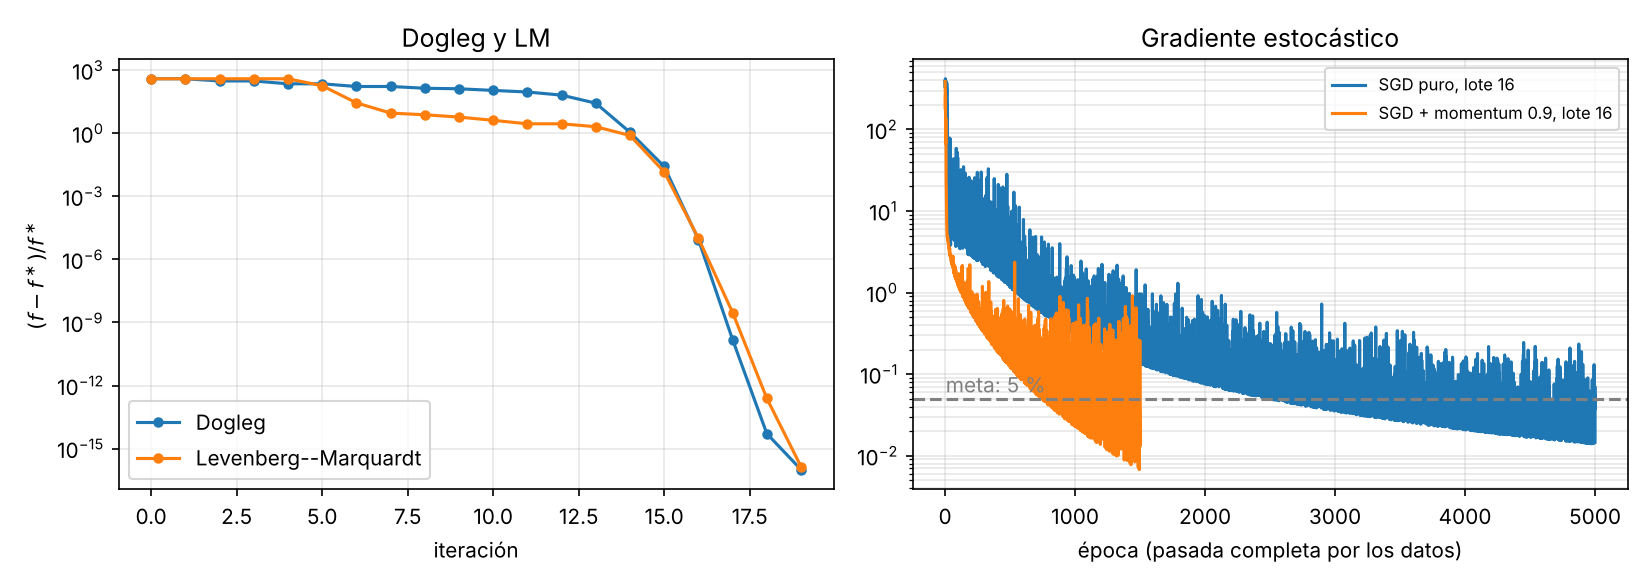
\includegraphics[width=\textwidth]{figs/fig_convergencia.png}
\caption{Convergencia. Dogleg y LM: convergencia superlineal al final. SGD: ruido de minilote y
meseta en torno al 1--2\,\%.}
\end{figure}

\subsection*{Parte C2: sensibilidad al punto inicial}
\begin{center}\small
\begin{tabular}{llrrrr}\toprule
& $\theta_0$ & \multicolumn{2}{c}{Dogleg} & \multicolumn{2}{c}{LM} \\
& & iter. & $f_{\rm final}$ & iter. & $f_{\rm final}$ \\\midrule
A & $(1, 1, 1, 0.5)$ & 20 & 0.1991 & 20 & 0.1991 \\
B & $(5, 5, 5, 5)$ & 171 & 2.0050 & 30 & 0.1991 \\
C & $(1, 0.3, 1, 0.35)$ & 16 & 0.1991 & 21 & 0.1991 \\
D & $(1, 0.1, 1, 2)$ & 8 & 0.1991 & 11 & 0.1991 \\
E & $(3, 0.5, 0.5, 0.05)$ & 8 & 0.1991 & 10 & 0.1991 \\
F & $(1, 1, 1, 1)$ & 132 & 2.0050 & 33 & 0.1991 \\
\bottomrule\end{tabular}

\end{center}
Observaciones:
\begin{itemize}
\item \textbf{B y F con Dogleg} terminan en $f=2.005$ en el punto $\tht\approx(1.864,\,0.178,\,1.864,\,0.178)$, donde
$a=c$ y $b=d$: las dos exponenciales coinciden y el modelo colapsa a $2a\,e^{-bt}$. El gradiente es $\approx10^{-6}$
(por eso Dogleg se detiene), $\mathbf B$ tiene \textbf{dos autovalores nulos} ($\sim10^{-14}$) y la
\textbf{Hessiana exacta tiene un autovalor $-142$}: es un \textbf{punto silla}, no un m\'inimo. La aproximaci\'on
de Gauss--Newton no ve esa curvatura negativa (es semidefinida positiva), y como $\mathbf B$ es singular el
Dogleg solo usa el paso de Cauchy, de modo que no puede escapar y avanza lentamente.
\item Desde el inicio simétrico exacto F, las iteraciones de LM tambi\'en permanecen sim\'etricas ($|a-c|=0$) durante
varias iteraciones; \textbf{LM sale del punto silla por amplificaci\'on del ruido num\'erico a lo largo de la
direcci\'on de curvatura negativa}, no por una garant\'ia te\'orica. Con asimetr\'ia peque\~na en $\tht_0$
(p.\,ej. $d_0=1+10^{-4}$) ambos m\'etodos convergen; con $10^{-2}$ Dogleg a\'un se queda cerca del silla
tras 500 iteraciones. Moraleja: verificar autovalores de la Hessiana exacta al terminar y no comenzar en
configuraciones sim\'etricas.
\item \textbf{Inicio D}: $(a,b)\leftrightarrow(c,d)$ intercambia los dos t\'erminos sin cambiar $y(t)$; por eso
D converge a $\tht^\ast$ \emph{permutado}, $(3.02,\,0.147,\,1.87,\,1.694)$, con el mismo $f^\ast$. Soluci\'on:
imponer la convenci\'on $b>d$ (reordenar los pares $(a,b)$, $(c,d)$ al reportar) o reparametrizar con $b=d+e^{\gamma}$.
\item \textbf{Inicio C} ($b\approx d$) deja $\mathbf B$ casi singular; ambos m\'etodos convergen sin problemas.
\end{itemize}

\begin{figure}[h]
\centering
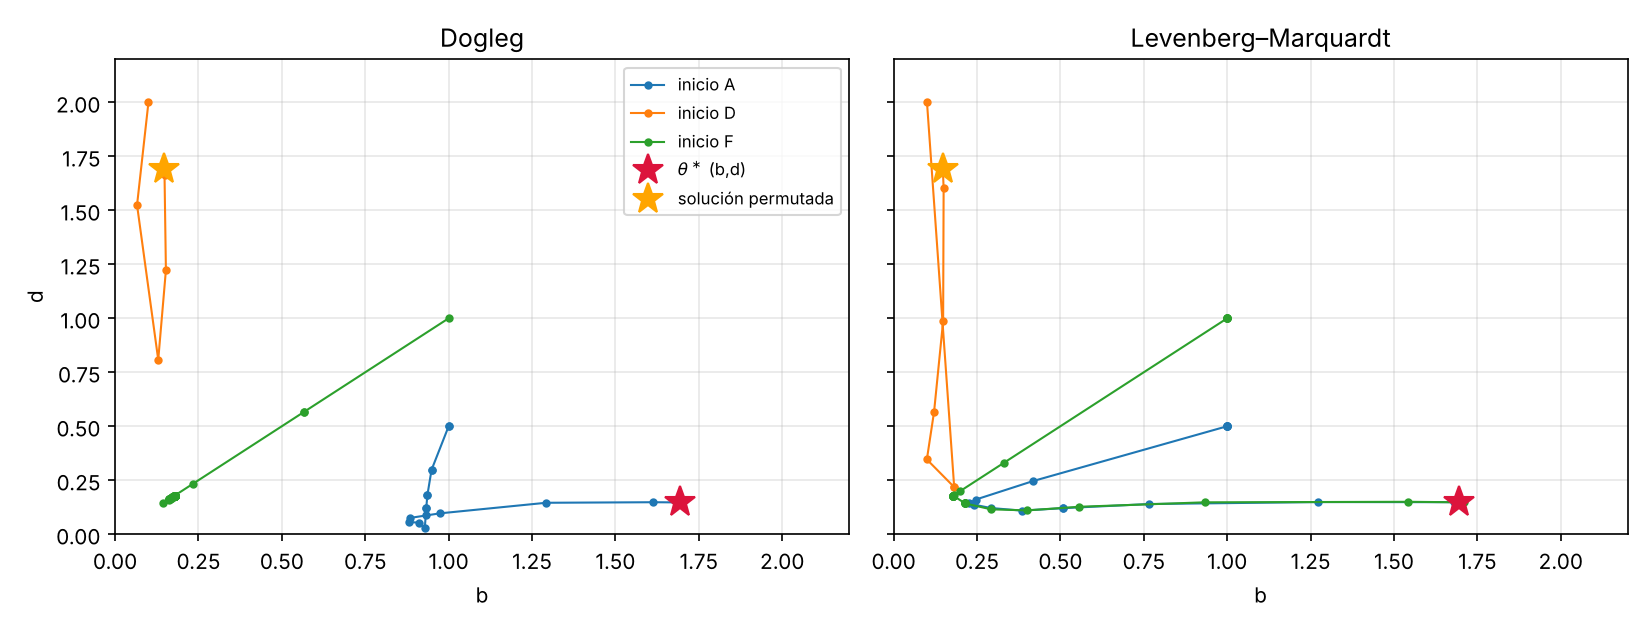
\includegraphics[width=\textwidth]{figs/fig_trayectorias_bd.png}
\caption{Trayectorias en el plano $(b,d)$. Dogleg desde F llega al punto sim\'etrico $b=d\approx0.18$; LM lo atraviesa.}
\end{figure}

\subsection*{Parte C3: gradiente estoc\'astico (3000 \'epocas, $\alpha_0=0.1$, $k_0=5000$)}
\begin{center}\small
\begin{tabular}{lrr}
\toprule
Configuraci\'on & pasos & $(f-f^\ast)/f^\ast$ final\\
\midrule
lote 150 (gradiente completo) & 3\,000 & 4.84\\
lote 16, paso decreciente & 30\,000 & 0.065\\
lote 4, paso decreciente & 114\,000 & 0.0086\\
lote 16, paso constante 0.1 & 30\,000 & 14.5 (oscila)\\
lote 16, paso constante 0.02 & 30\,000 & 0.097\\
\bottomrule
\end{tabular}
\end{center}
El lote completo \emph{no} es mejor: con las mismas \'epocas (igual c\'omputo de datos) hace 10 veces menos pasos
que el lote 16. El paso constante grande oscila y no converge; uno peque\~no converge pero lento; el decreciente combina
ambas. Momentum $\beta=0.9$ con $\alpha_0=0.01$ llega al 1.3\,\% en 15\,000 pasos. La causa de la lentitud es el mal
condicionamiento: los autovalores de $\mathbf B=\mathbf J^\top\mathbf J$ en $\tht^\ast$ son
$0.25,\;0.98,\;11.1,\;5.4\times10^{3}$, es decir $\kappa=2.1\times10^4$. Para el costo medio $f/n$ el paso estable
cumple $\alpha<2n/\lambda_{\max}(\mathbf B)\approx0.055$ (por eso el paso constante 0.1 oscila y 0.02 no), y
la direcci\'on de curvatura menor se contrae solo por un factor $1-\alpha\lambda_{\min}/n\approx1-3\times10^{-5}$
por paso (con $\alpha=0.02$): decenas de miles de pasos para reducir el error en ella por un factor $e$.
Dogleg y LM, en cambio, reescalan con $\mathbf B$ y no sufren por $\kappa$. SGD es la mejor opci\'on cuando $n$ es enorme (millones de datos), cada
iteraci\'on de LM costar\'ia demasiado y basta precisi\'on moderada (aprendizaje autom\'atico).

\begin{figure}[h]
\centering
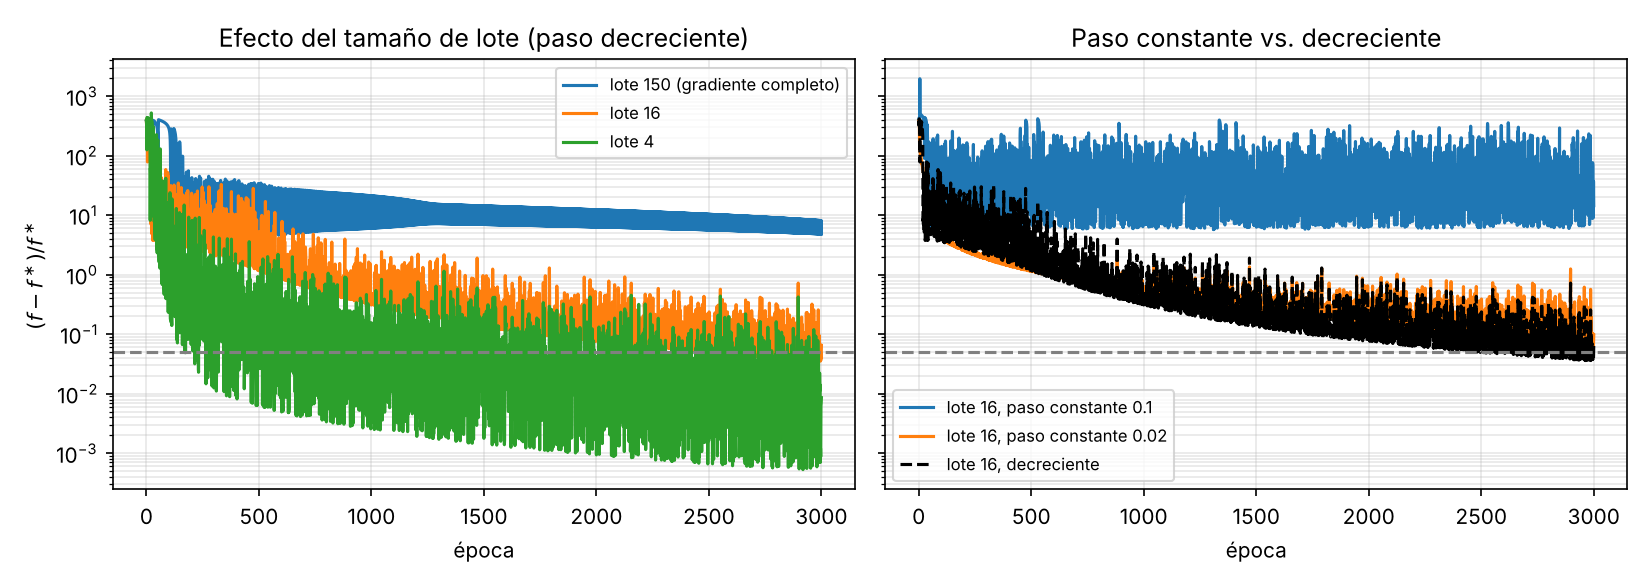
\includegraphics[width=\textwidth]{figs/fig_sgd_parametros.png}
\caption{Efecto del lote (izquierda) y del paso (derecha).}
\end{figure}

\subsection*{Parte D: incertidumbre en $\tht^\ast$}
\begin{center}\small
\begin{tabular}{lrrrr}
\toprule
& $a$ & $b$ & $c$ & $d$\\
\midrule
$\tht^\ast$ & 1.870 & 1.694 & 3.020 & 0.1471\\
desv.\ est. & 0.050 & 0.101 & 0.032 & 0.0016\\
IC 95\,\% ($\pm1.98\,$sd) & $\pm0.099$ & $\pm0.201$ & $\pm0.064$ & $\pm0.0031$\\
error relativo (sd/valor) & 2.7\,\% & 6.0\,\% & 1.1\,\% & 1.1\,\%\\
\bottomrule
\end{tabular}
\end{center}
Los cuatro valores verdaderos caen dentro de sus intervalos. Correlaciones: $\mathrm{corr}(c,d)=0.89$,
$\mathrm{corr}(b,c)=0.67$, $\mathrm{corr}(b,d)=0.55$, $\mathrm{corr}(a,c)=-0.44$, $\mathrm{corr}(a,d)=-0.41$;
$\kappa(\mathbf J^\top\mathbf J)=2.1\times10^4$. La tasa r\'apida $b$ es la peor determinada (error relativo $6$\,\%)
porque el transitorio r\'apido ocupa pocos minutos de $[0,20]$ y solo unos pocos datos lo observan; $c$ y $d$
est\'an fuertemente correlacionados porque un exceso de amplitud lenta se compensa con una tasa un poco mayor.

Efecto del ruido (mismos $t_i$, $\sigma$ creciente):
\begin{center}\small
\begin{tabular}{rrrrr}
\toprule
$\sigma$ & sd($a$) & sd($b$) & sd($c$) & sd($d$)\\
\midrule
0.05 & 0.050 & 0.101 & 0.032 & 0.0016\\
0.2 & 0.209 & 0.501 & 0.112 & 0.0056\\
0.5 & 0.548 & 1.557 & 0.246 & 0.0127\\
\bottomrule
\end{tabular}
\end{center}
Las desviaciones crecen aproximadamente $\propto\sigma$ ($\sigma\to4\sigma$ multiplica sd$(a)$ por $4.2$). Para $b$ crece
\emph{m\'as} que proporcionalmente (sd pasa de 0.10 a 1.56 al multiplicar $\sigma$ por 10) y la estimaci\'on se
desplaza ($\hat b=1.69,\,2.17,\,3.00$): con ruido alto la tasa r\'apida deja de ser identificable.

\section{Puntos a revisar al calificar}
\begin{itemize}
\item \textbf{Dogleg:} que no use el paso de Newton cuando $\mathbf B$ es singular (si lo hace, el modelo puede
subir y $\rho_k<0$ constante); que $\rho_k$ use el modelo (no la funci\'on) en el denominador; que rechace el
paso si $\rho_k\le0$.
\item \textbf{LM:} escalado con $\mathrm{diag}(\mathbf B)$ (las columnas de $\mathbf J$ difieren en varios \'ordenes de
magnitud: $\partial r/\partial d\sim t$ crece con $t$); $\lambda$ no puede crecer sin l\'imite (parar por paso
despreciable); relaci\'on $\lambda\uparrow\Leftrightarrow\Delta\downarrow$.
\item \textbf{SGD:} que el gradiente del lote est\'e dividido por $m$ (si no, $\alpha_0$ depende del lote); que
comparen por \'epocas o evaluaciones de datos, no por pasos.
\item \textbf{C2:} que no concluyan ``Dogleg es peor'' sin diagnosticar el punto silla con la Hessiana exacta, y
que no atribuyan el escape de LM a una garant\'ia que no existe.
\item \textbf{Variantes de datos:} cada estudiante tiene $\tht_{\rm real}$ distinto ($\pm10$\,\%); los valores de
este documento no coinciden con los suyos, pero las conclusiones cualitativas s\'i. Compara $\tht^\ast$ con la
tabla \texttt{verdad\_parametros.csv}.
\end{itemize}

\section{C\'omo generar los datos de cada estudiante}
\begin{verbatim}
python generar_datos.py 1017123456 1020333444 ...     # una semilla por documento
python generar_datos.py --lista documentos.txt        # uno por linea
\end{verbatim}
Se crea \texttt{datos\_estudiantes/datos\_<doc>.csv} para cada uno y
\texttt{verdad\_parametros.csv} (no se entrega a los estudiantes).
\end{document}
